\documentclass{article}

\title{Assignment 7\\\normalsize{Advanced Programming}}
\author{Jordi Riemens\\Thomas Churchman}

\usepackage[utf8]{inputenc}
\usepackage{listings}
\lstset{basicstyle=\ttfamily}

\usepackage{graphicx}
\graphicspath{ {images/} }

\begin{document}
	\maketitle
	
    For the sake of brevity, we will mainly describe the decisions made in the more interesting parts of our system.
    A list of screenshots can be found in the appendix.
    
	\section{Proposal mechanism}
    For the proposal mechanism, we took inspiration from \texttt{datumprikker.nl}.
    On this site, the proposal maker first fills in general details about the appointment. In our case, this is the title, duration (we assume this is fixed) and participants.
    Next, the user chooses the dates on which the appointment could be planned, but not the times. Afterwards, for each date, the user gets to fill in a list of times.
    As on the site, for a mix of convenience and flexibility, there is a ``copy times from the first date" button, which copies all proposed times from the uppermost date,
    and fills them in for all other dates, as well, so that if the proposed times do not depend on the date, filling them in is quick.
    
    When the proposal is created, it is stored in a shared database, and an empty list of responses is created in a separate shared database.
    Furthermore, an invitation task is created for all participants, and for the owner a proposal management task is created.
    In the proposal management task, all responses given so far are listed, and the owner can choose between the proposed date-times, and then click \emph{Schedule} to create an actual appointment for all participants.
    In this case, the proposal and its response list are removed from their respective databases to invalidate remaining proposal tasks.
    As the response list is in a shared database, we let the displayed response list on the proposal management task update in real time, and the user can close the task and revisit it later.
    
    When a user opens an invitation, we first check in the database whether the proposal still exists.
    If the proposal is still ongoing, we display the proposal and offer a checklist to choose which times are suitable, which is added to the corresponding entry in the response database.
    If the proposal no longer exists, then an appointment has already been scheduled, so we display the scheduled appointment instead.
    This way, the user is notified that a date-time proposal process has taken place, although they were not in time to indicate their preferences.
    
    \section{Appointment creation and parallel tasks}
	When an appointment is created (either from \emph{Make appointments} or from scheduling from a \emph{Manage proposal} task), a parallel scheduler task is detached.
	This scheduler task waits until the appointment start time.
	Once the appointment start time is reached, the scheduler task launches in parallel one task per participant that displays the appointment to that participant.
	These viewing tasks wait until the appointment end time and then finish.
	The tasks are detached, and not embedded, as an embedded parallel task launched from a transient workflow is stopped once the transient workflow is closed.
    
    \section{Canceling tasks}
	We wanted to implement a method of gracefully canceling a task.
	For example, when working on the \emph{Manage proposal} task, a user might wish to cancel managing the proposal.
	We have attempted to include a cancellation action, but have not been able to get this to work nicely with the workflow framework.
	We tried returning various values, such as \lstinline|return ()|, \lstinline|throw "Cancel"|, and have tried changing the return type, as well as ending with an interaction task (\lstinline|viewInformation "Success" [] "Cancelled"|), but these either do not achieve the desired effect, or simply crash the iTasks GUI.
	In the current version of iTasks (2017-11-08 nightly), the ``Close" button supplied by the iTasks worklist framework also crashes the GUI.
	As such, we assume there is a bug in the current iTasks version that prevents such buttons from working as intended.
    
    \section{Cosmetic types}
	We were not satisfied with the way appointments, proposals and their responses were displayed, where in particular the default user display was unnecessarily detailed; only a name was needed for our purposes.
    Unfortunately, to be able to use \lstinline|viewInformation| to display them in a nicer way, we need a destination type with an \lstinline|iTask| implementation.
    Furthermore, simple tuples do not work, because they distribute layout space evenly; this is not what we want, as a list of participants requires more space than a title.
    Thus, we created `cosmetic types' for appointments, proposals and proposal responses purely for display purposes, resulting in a more readable participant list and/or response list.
	
	\newpage
	\appendix
	\section{Screenshots}
	
	\begin{figure}[h!]
		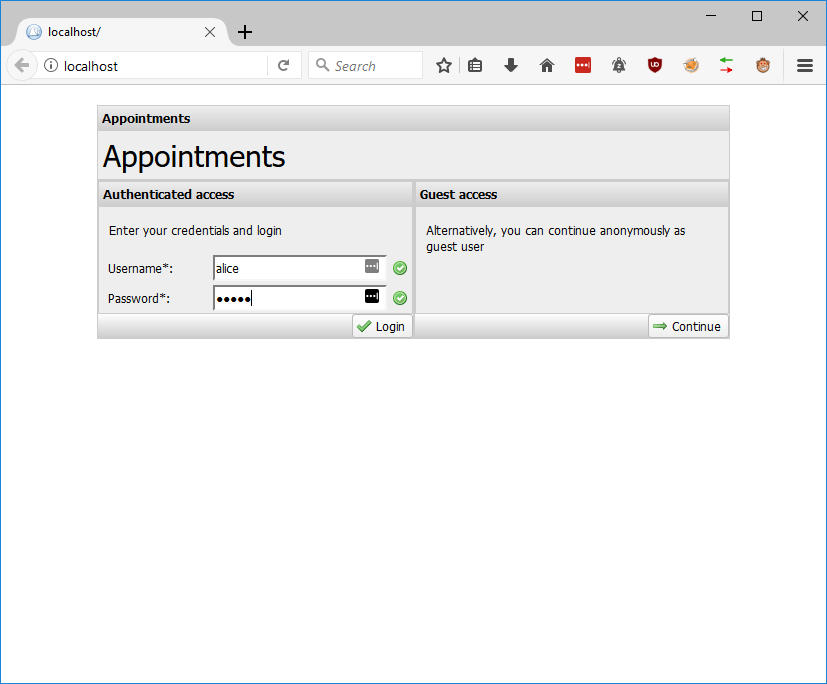
\includegraphics[width=\textwidth]{01_login}
		\caption{Logging in}
	\end{figure}
	
	\begin{figure}[h!]
		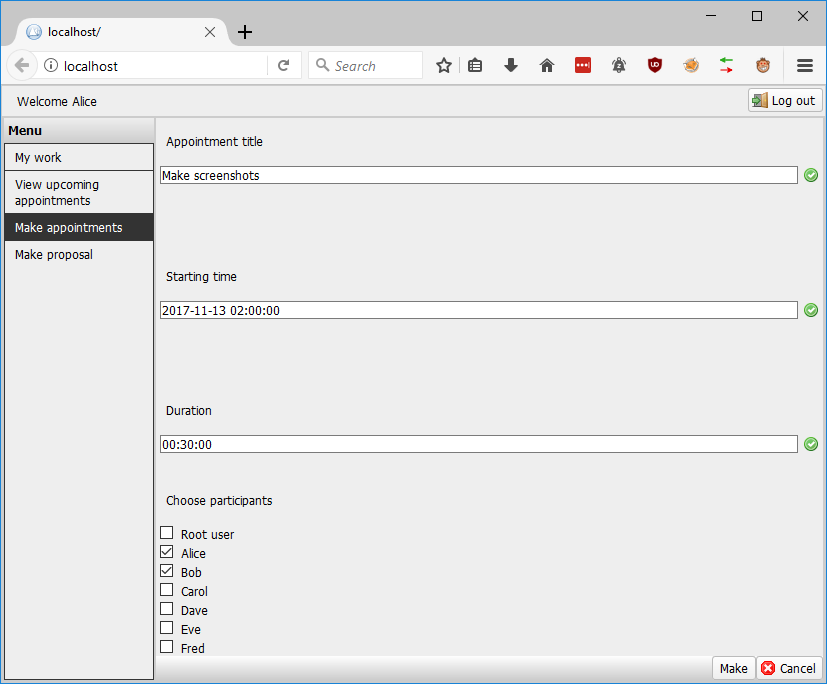
\includegraphics[width=\textwidth]{02_make_appointment}
		\caption{Making an appointment}
	\end{figure}
	
	\begin{figure}[h!]
		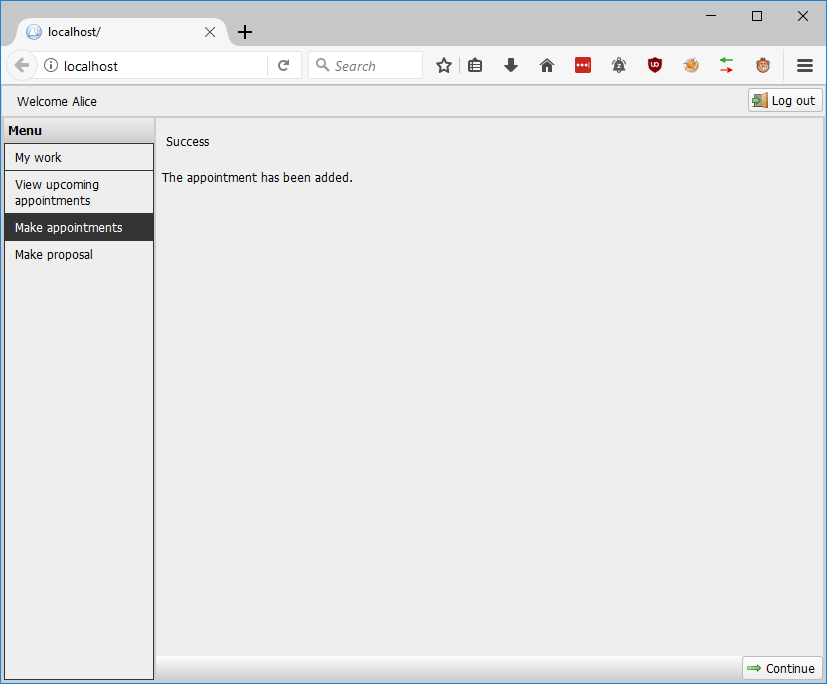
\includegraphics[width=\textwidth]{03_appointment_added}
		\caption{Appointment added}
	\end{figure}
	
	\begin{figure}[h!]
		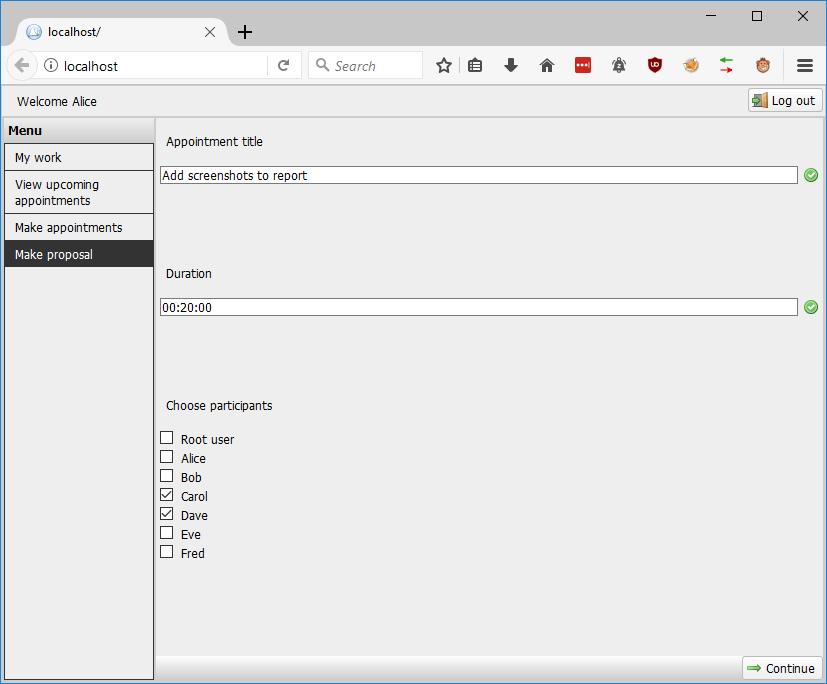
\includegraphics[width=\textwidth]{04_make_proposal}
		\caption{Proposing an appointment}
	\end{figure}
	
	\begin{figure}[h!]
		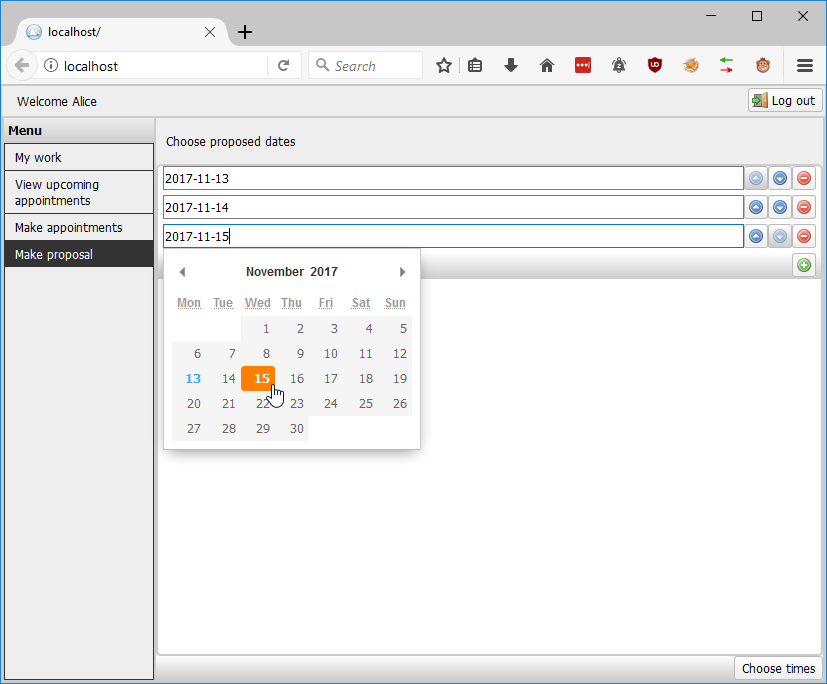
\includegraphics[width=\textwidth]{05_make_proposal_choose_dates}
		\caption{Proposing an appointment: choose dates}
	\end{figure}
	
	\begin{figure}[h!]
		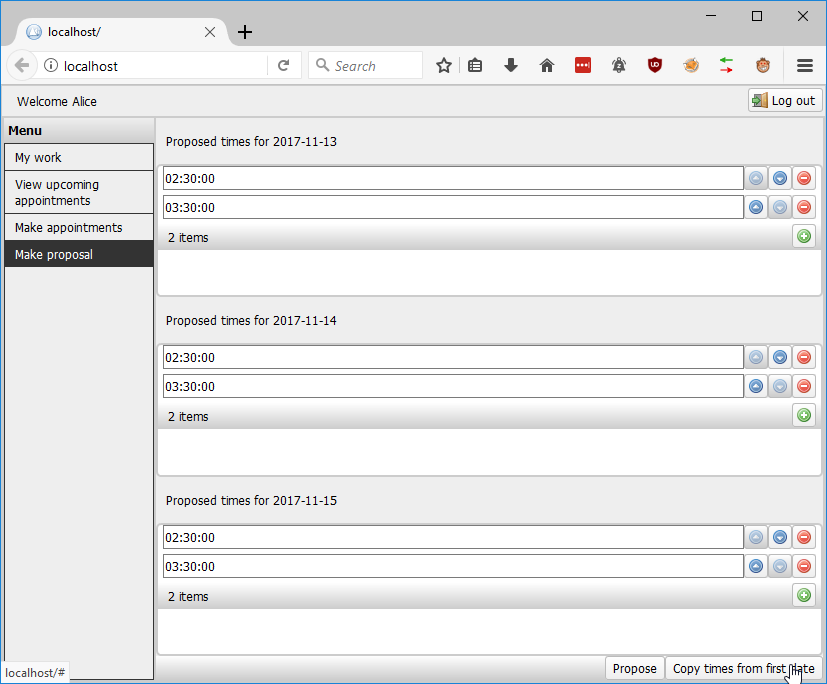
\includegraphics[width=\textwidth]{06_make_proposal_choose_times}
		\caption{Proposing an appointment: choose times}
	\end{figure}
	
	\begin{figure}[h!]
		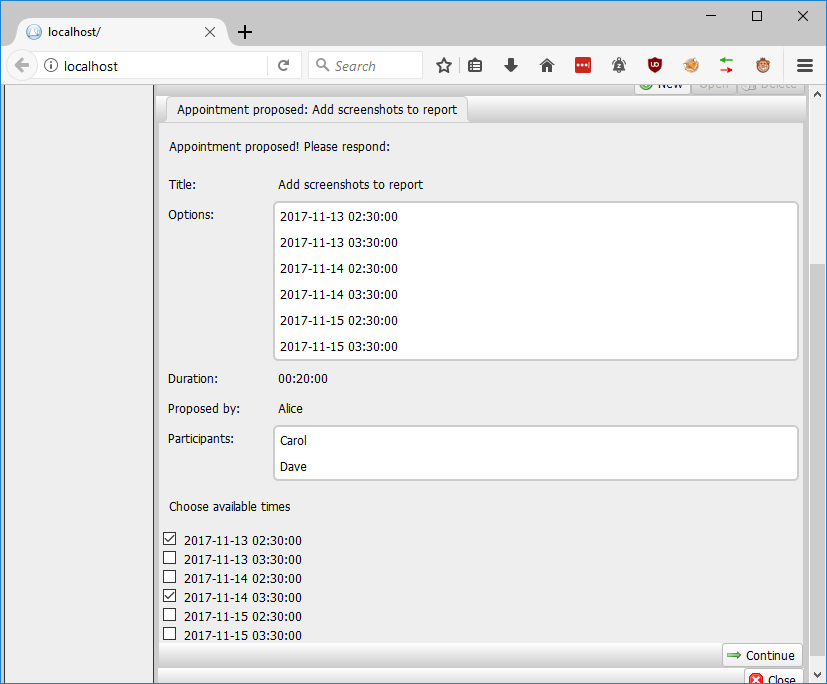
\includegraphics[width=\textwidth]{07_dave_choose_proposal_date_times}
		\caption{Viewing the appointment invitation: choose available dates and times}
	\end{figure}
	
	\begin{figure}[h!]
		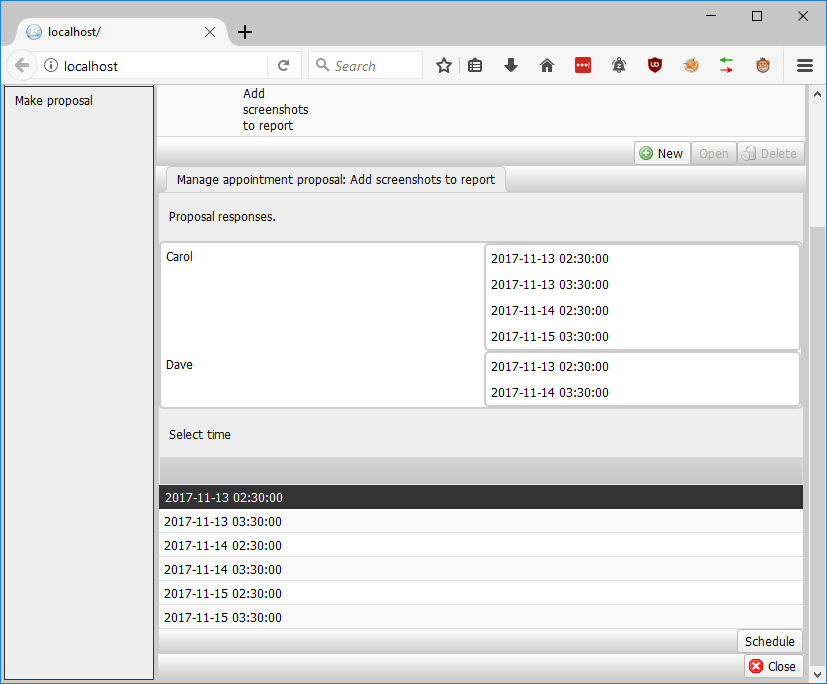
\includegraphics[width=\textwidth]{08_manage_proposal}
		\caption{Managing the proposal: see responses and schedule}
	\end{figure}
	
	\begin{figure}[h!]
		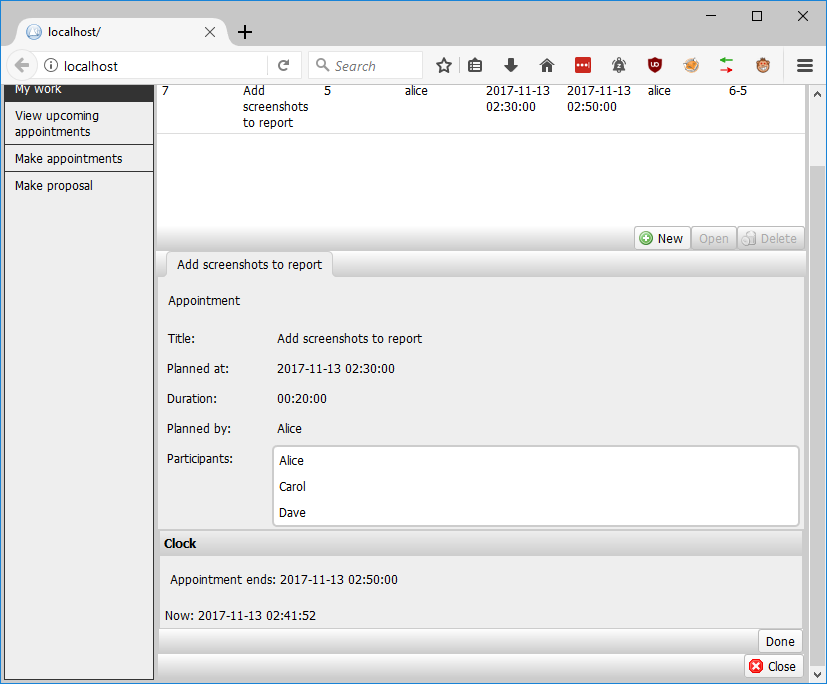
\includegraphics[width=\textwidth]{09_view_appointment}
		\caption{Viewing an active appointment}
	\end{figure}
	
	\begin{figure}[h!]
		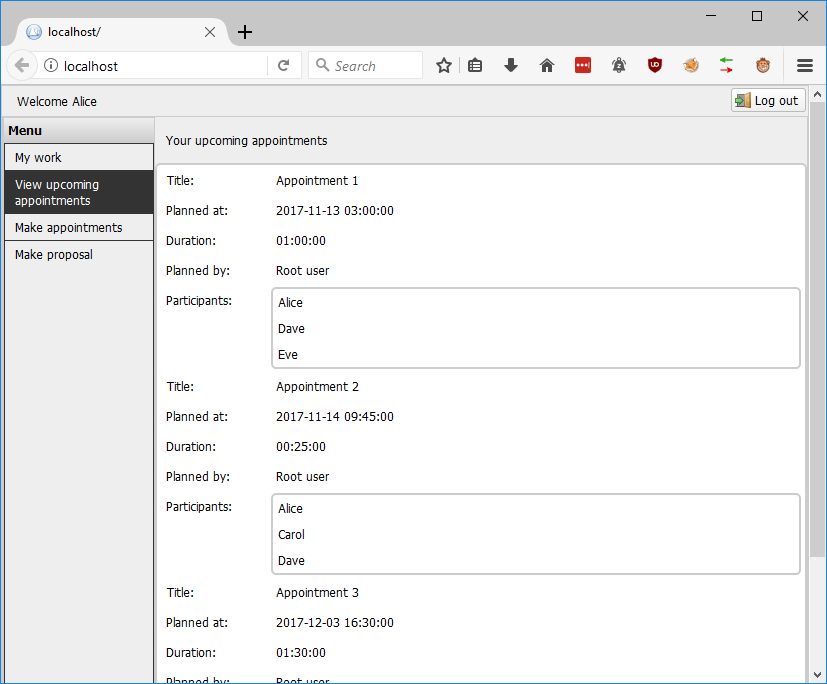
\includegraphics[width=\textwidth]{10_upcoming_appointments}
		\caption{Looking at upcoming appointments}
	\end{figure}
	
\end{document}
